\documentclass{article}

\usepackage{amsmath}
\usepackage{amsthm}
\usepackage{amssymb}
\usepackage{amsfonts}
\usepackage{tikz}
\usepackage{multicol}
\usepackage{xcolor}
\usepackage{bbm}
\usepackage[utf8]{inputenc}
\usepackage[a4paper, margin=1in]{geometry}

\theoremstyle{definition}

\newtheorem{theorem}{Theorem}[section]
\newtheorem{corollary}{Corollary}[section]
\newtheorem{prop}{Proposition}[section]
\newtheorem{lemma}[theorem]{Lemma}
\newtheorem{dd}{Definition}[section]

\DeclareMathOperator{\tr}{tr}
\DeclareMathOperator{\diam}{diam}

\begin{document}

\section*{\LARGE{Graphs and their products.}}

\section{Basic definitions and theorems.}

\subsection{A graph}

\begin{dd}
    A graph is an ordered set $G = \left( V(G),\ E(G),\ \delta_G \right)$ comprising of a set of vertices $V(G)$ and a set of edges $E(G)$ and a function $\delta_G: E(G) \to V(G) \times V(G)$.
\end{dd}

\subsection{Edges and verices}

\begin{dd}
    Each edge $e \in E(G)$ starts at a vertex denoted by $i(e) \in V(G)$ and terminates at a vertex denoted by $t(e) \in V(G)$. $\delta_G(e) = \left( i(e),\ t(e) \right)$
\end{dd}

\begin{dd}
    Let graph $G = \left( V(G), E(G) \right)$. Vertices $a, b \in V(G)$ are incident to $e \in E(G)$ and are adjacent (each other's neighbors) if there exists an edge $e \in E(G)$ such that $e = ab$.
\end{dd}

\begin{dd}
    A simple graph has no multiple edges and no loops.
\end{dd}

\subsection{Basic facts}

\begin{enumerate}
    \item $G = \left( V(G),\ E(G) \right)$ is finite if $V(G)$ is finite
    \item $O = \left( V(O),\ E(O) \right)$ is an empty graph is $V(O) = \emptyset$
    \item $G = \left( V(G),\ E(G) \right)$ is nontrivial if $|V(G)| > 1$
    \item $|V(G)|$ is called order and $|E(G)|$ is called size
\end{enumerate}

\subsection{Types of graphs}

\begin{itemize}
    \item{
        \textbf{Complete graph $K_n$} \\
        A graph with $n$ vertices, where any two are connected by an edge. \\
        Order: $|V(K_n)| = n$, size: $|E(K_n)| = \binom{n}{2} = \frac{n(n-1)}{2}$

        \begin{itemize}
            \item {
                $K_5$ \par
                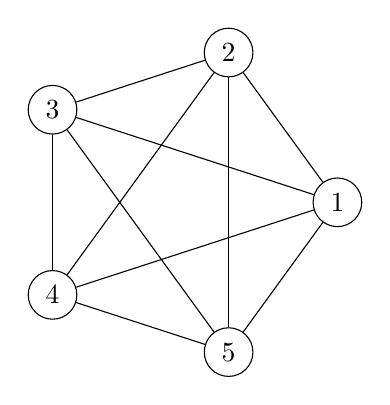
\begin{tikzpicture}[every node/.style={circle, draw, minimum size=0.5cm}]
                    \foreach \angle/\label in {0/1, 72/2, 144/3, 216/4, 288/5} {
                        \node (\label) at (\angle:2cm) {\label};
                    }
        
                    \draw (1) -- (2);
                    \draw (1) -- (3);
                    \draw (1) -- (4);
                    \draw (1) -- (5);
                    \draw (2) -- (3);
                    \draw (2) -- (4);
                    \draw (2) -- (5);
                    \draw (3) -- (4);
                    \draw (3) -- (5);
                    \draw (4) -- (5);
                \end{tikzpicture}
            }
        \end{itemize}
    }

    \item{
        \textbf{Complete bipartite graph $K_{n,m}$} \\
        A graph with $n$ points in one part, $m$ points in another part, where any two points from different parts are connected by an edge. \\
        Order: $|V(K_{n,m})| = n + m$, size: $|E(K_{n,m})| = n \cdot m$
    
        \begin{itemize}
            \item {
                $K_{3,3}$ \par
                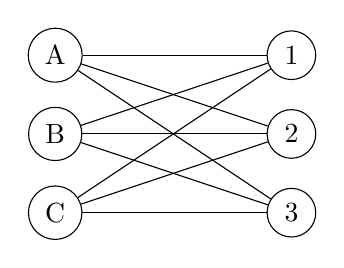
\begin{tikzpicture}[every node/.style={circle, draw, minimum size=0.5cm}]
                    \node (A) at (0, 2) {A};
                    \node (B) at (0, 1) {B};
                    \node (C) at (0, 0) {C};
                    \node (1) at (3, 2) {1};
                    \node (2) at (3, 1) {2};
                    \node (3) at (3, 0) {3};
                
                    \draw (A) -- (1);
                    \draw (A) -- (2);
                    \draw (A) -- (3);
                    \draw (B) -- (1);
                    \draw (B) -- (2);
                    \draw (B) -- (3);
                    \draw (C) -- (1);
                    \draw (C) -- (2);
                    \draw (C) -- (3);
                \end{tikzpicture}
            }
        \end{itemize}
    }

    \item{
        \textbf{Path graph $P_n$} \\
        A graph with $n$ vertices $\{ v_1, v_2, \dots, v_n \}$ and $n - 1$ edges $\{ v_1v_2, v_2v_3, ..., v_{n-1}v_n \}$. \\
        Order: $|V(P_n)| = n$, size: $|E(P_n)| = n - 1$

        \begin{itemize}
            \item {
                $P_5$ \par
                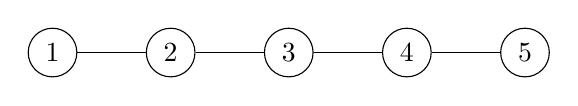
\begin{tikzpicture}[every node/.style={circle, draw, minimum size=0.5cm}]
                    \node (A) at (0,0) {1};
                    \node (B) at (1.5,0) {2};
                    \node (C) at (3,0) {3};
                    \node (D) at (4.5,0) {4};
                    \node (E) at (6,0) {5};
                
                    \draw (A) -- (B);
                    \draw (B) -- (C);
                    \draw (C) -- (D);
                    \draw (D) -- (E);
                \end{tikzpicture}
            }
        \end{itemize}
    }

    \item{
        \textbf{Cycle graph $C_n$} \\
        A graph with $n$ vertices $\{ v_1, v_2, \dots, v_n \}$ and $n$ edges $\{ v_1v_2, v_2v_3, \dots, v_{n-1}v_n, v_nv_1 \}$. \\
        Order: $|V(C_n)| = n$, size: $|E(C_n)| = \begin{cases}
            n & \text{for}\ n > 2 \\
            n - 1 & \text{for}\ n \leq 2
        \end{cases}$

        \begin{itemize}
            \item {
                $C_8$ \par
                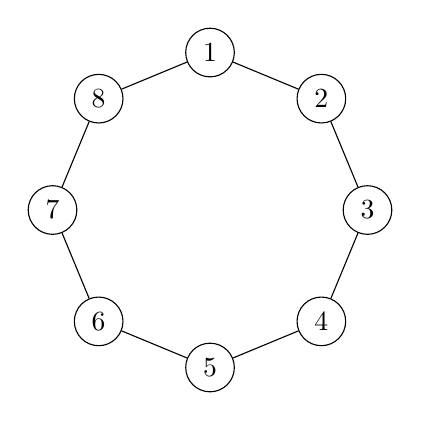
\begin{tikzpicture}[every node/.style={circle, draw, minimum size=0.5cm}]
                    \node (A) at (90:2cm) {1};
                    \node (B) at (45:2cm) {2};
                    \node (C) at (0:2cm)  {3};
                    \node (D) at (-45:2cm) {4};
                    \node (E) at (-90:2cm) {5};
                    \node (F) at (-135:2cm) {6};
                    \node (G) at (180:2cm) {7};
                    \node (H) at (135:2cm) {8};
                
                    \draw (A) -- (B);
                    \draw (B) -- (C);
                    \draw (C) -- (D);
                    \draw (D) -- (E);
                    \draw (E) -- (F);
                    \draw (F) -- (G);
                    \draw (G) -- (H);
                    \draw (H) -- (A);
                \end{tikzpicture}
            }
        \end{itemize}
    }
\end{itemize}

\subsection{Degrees, subgraphs, etc.}

\begin{dd}
    A degree of a vertex $v \in V(G)$ is the number of edges incident with $v$.
\end{dd}

\begin{dd}
    A graph $G' = \left( V(G'), E(G') \right)$ is a subgraph of graph $G = \left( V(G), E(G) \right)$ if $V(G') \subseteq V(G)$ and $E(G') \subseteq E(G)$. $G'$ is a spanning subgraph of $G$ if $V(G') = V(G)$.
\end{dd}

\begin{lemma}[Handshaking lemma]
    Let $G = \left( V(G), E(G) \right)$ be a graph. Let $V(G) = \{ v_1, \dots, v_n \}$. Then $\sum\limits_{i = 1}^n \deg v_i = 2 \cdot |E(G)|$ or $\sum\limits_{i = 1}^n \deg v_i = 2 \cdot (|E(G)| + |L(G)|)$ where $L(G)$ is the set of loops.
\end{lemma}

\begin{dd}
    $G$ is a regular graph if all its vertices have the same degree $r$. We can also say that $G$ is $r$-regular. 3-regular graphs are called cubic graphs. 
\end{dd}

\begin{dd}
    We can say that graphs $G$ and $H$ are isomorphic, or $G \cong H$, if there exists a bijection $\phi: V(G) \to V(H)$ such that $\phi(u)\phi(v) \in E(H) \iff uv \in E(G)$.
\end{dd}

\begin{dd}
    Let $G = \left( V(G), E(G) \right)$ be a graph. The complement graph $\overline{G}$ is a graph such that $V(\overline{G}) = V(G)$ and $ab \in E(\overline{G}) \iff ab \notin E(G)$.
\end{dd}

\begin{dd}
    Let $G$ and $H$ be graphs. Homomorphism consists of a pair of maps $\Phi: V(G) \to V(H)$ and $\Psi: E(G) \to E(H)$ such that $i(\Psi(e)) = \Phi(i(e))$ and $t(\Psi(e)) = \Phi(t(e))$ for all edges $e \in E(G)$. We write $(\Phi, \Psi): G \to H$.
    \begin{itemize}
        \item If both $\Phi$ and $\Psi$ are $1-1$ it's called \textbf{graph embedding}.
        \item If both $\Phi$ and $\Psi$ are bijective it's called \textbf{graph isomorphism}.
    \end{itemize}
\end{dd}

\begin{dd}[Adjacency matrix]
    Let $G$ be a graph with a finite enumarated set $V(G)$. Let $M_{I,J}$ denote the number of edges in $G$ with initial state $I$ and terminal state $J$ for vertices $I, J \in V(G)$. The adjacency matrix of $G$ is $M = [M_{I,J}]$ and its formation from $G$ is denoted by $M = M(G)$ or $M = M_G$.
\end{dd}

\subsection{Walks, paths, etc.}

\begin{dd}
    Let $(v_0, \dots, v_n)$ be a sequence of vertices in $G$ such that there exists $e_i = v_{i-1}v_i$ for $i = 1, \dots, n$. The sequence is called \textbf{walk}. \\
    If $v_0 = v_n$, it's called \textbf{closed walk}.
\end{dd}

\begin{dd}
    A walk for which all edges $e_i$ are distinct is called \textbf{trail}. \\
    If $v_0 = v_n$, it's called \textbf{closed trail} or \textbf{tour}.
\end{dd}

\begin{dd}
    If all vertices in a trail are distinct, it's called \textbf{path}. \\
    A closed trail for $n \geq 3$ for which all vertices $v_i$ are distinct (except $v_0 = v_n$) is called \textbf{cycle}.
\end{dd}

\begin{lemma}
    A connected graph of $n$ vertices has at least $n - 1$ edges.
\end{lemma}

\subsection{Trees}

\begin{dd}
    An acyclic graph (one not containing any cycles) is called \textbf{forest}.
\end{dd}

\begin{dd}
    A leaf is a vertex of degree 1 in a forest.
\end{dd}

\begin{dd}
    A \textbf{tree} is a connected forest.
\end{dd}

\noindent The following statements are equivalent:
\begin{itemize}
    \item $T$ is a tree
    \item $T$ is an acyclic graph with $n - 1$ edges
    \item $T$ is a connected graph with $n - 1$ edges
    \item Any two vertices of $T$ are linked by a unique path in $T$
\end{itemize}

\subsection{Eulerian and Hamiltonian graphs}

\begin{dd}
    An \textbf{Eulerian trail} of graph $G$ is a trail which contains each edge of $G$ exactly once. If the trail is closed, it's called \textbf{Euler tour}.
\end{dd}

\begin{dd}
    A graph is Eulerian if it admits Euler tour.
\end{dd}

\begin{lemma}
    Let $G$ be a graph such that $\deg v \geq 2$ for any vertex $v \in V(G)$. Then $G$ contains a closed trail.
\end{lemma}

\begin{theorem}
    A connected finite graph is Eulerian $\iff$ $\forall v \in V(G):\ 2|\deg v$.
\end{theorem}

\begin{corollary}
    A connected finite graph $G$ has an Euler trail from a vertex $x \in V(G)$ to a vertex $y \in V(G)$ ($x \neq y$) $\iff$ $x$ and $y$ are the only vertices of odd degrees. 
\end{corollary}

\begin{dd}
    \textbf{Hamiltonian (traceable) path} is a path that visits each vertex exactly once. \textbf{Hamiltonian cycle} is a cycle which contains each vertex exactly once.
\end{dd}

\begin{dd}
    A graph is Hamiltonian if it admits Hamiltonian cycle.
\end{dd}

\subsection{Dirac, Ore and other theorems}

\begin{theorem}[Dirac's]
    Let $G$ be a graph with $n \geq 3$ vertices. If each vertex of $G$ has a degree at least $\frac{n}{2}$, then $G$ is Hamiltonian.
\end{theorem}

\begin{theorem}[Ore's]
    Let $G$ be a graph with $n \geq 3$ vertices. If $\deg u + \deg v \geq n$ for any two non-adjacent vertices $u, v \in V(G)$, then $G$ is Hamiltonian.
\end{theorem}

\begin{dd}[Closure of a graph]
    Let $G$ be a graph with $n$ vertices. If $G$ contains non-adjacent vertices $u, v \in V(G)$ such that $\deg u + \deg v \geq n$, we add the edge $uv$ to $G$. We continue until we get a graph $[G]$ in which for any two non-adjacent vertices $x, y \in V([G])$ we always have $\deg x + \deg y < n$. $[G]$ is the closure of $G$.
\end{dd}

\begin{theorem}[Bondy and Chvatal]
    A graph $G$ is Hamiltonian $\iff$ $[G]$ is Hamiltonian.
\end{theorem}

\begin{theorem}[Rachman and Kaykobad]
    A simple graph $G$ with $n$ vertices has a Hamiltonian path if for any non-adjacent vertex pairs the sum of their degrees and their shortest path length is greater than $n$.
\end{theorem}

\newpage
\section{Planar graphs, graph products and graph colouring.}

\subsection{Geometric graphs}

\begin{dd}
    Let $E$ be the set of line segments in 3-dimensional euklidean space, $V$ be the set of end points of those segments. A graph $G = (V, E)$ is called geometric if any two line segments in $E$ are disjoint, or have one of their end points in common.
\end{dd}

\begin{lemma}
    Every graph is isomorphic to a geometric graph.
\end{lemma}

\begin{dd}
    Geometric graph is a \textbf{plane} if all of its line segments lie in one plane. Any graph isomorphic to a plane graph is called \textbf{planar}.
\end{dd}

\begin{dd}
    Let $G = (V, E)$ be planar. The remainder $\mathbb{R}^2 \setminus G$ splits into a number of connected open regions. Closure of such a region is called a \textbf{face}.
\end{dd}

\begin{theorem}[Euler's formula]
    Let $G$ be a connected planar graph with $n$ vertices, $m$ edges and $f$ faces. Then the following equation holds: $$ n - m + f = 2 $$
\end{theorem}

\begin{corollary}
    Let $G$ be a connected planar graph with $n \geq 3$ vertices and $m$ edges. Then $m \leq 3n - 6$.
\end{corollary}

\subsection{Adjacency matrix and its usage}

\begin{dd}
    The matrix $M = [a_{ij}]_{n \times n}$ where $a_{ij}$ is the number of edges between vertices $v_i$ and $v_j$ is called the \textbf{adjacency matrix}.
\end{dd}

\begin{prop}
    Let $G$ be a graph with adjacency matrix $M$. Let $k \geq 0$.
    \begin{enumerate}
        \item The number of walks of length $k$ from $v_i$ to $v_j$ is $M^k_{ij}$ - the $(i, j)$th entry of $M^k$.
        \item The number of closed walks of length $k$ is $\tr(M^k)$
    \end{enumerate}
\end{prop}

\subsection{Distances}

\begin{dd}
    Let $G$ be a simple graph. The distance function $d_G: V(G) \times V(G) \to \mathbb{R}$ between two verices can be defined as follows: \\
    $d_G(u, v) = \begin{cases}
        \text{length of the shortest path between $u$ and $v$} & u \neq v \\
        0 & u = v \\
        \infty & \text{no path between $u$ and $v$}
    \end{cases}$
\end{dd}

\begin{dd}
    The diameter of a graph $G$ is defined as follows: $\diam G = \max\limits_{u, v \in V(G)} d_G(u, v)$.
    \begin{itemize}
        \item $\diam K_n = 1$
        \item $\diam P_n = n - 1$
        \item $\diam H_n = n$
        \item $\diam C_n = \left\lfloor \frac{n}{2} \right\rfloor$
    \end{itemize}
\end{dd}

\subsection{Hamming metric space and hamming graphs}

\begin{dd}
    Let $A = \{a_1, \dots, a_m\}$ be the alphabet set, $H_n(A) = \{(x_1, \dots, x_n): x_i \in A\}$. Let $d_{H_n}$ be the metric, defined as the number of positions with different symbols. The pair $\left( H_n(A), d_{H_n} \right)$ is called the \textbf{hamming metric space}.
\end{dd}

\begin{dd}
    A Hamming graph is the pair $H_n = \left( H_n(\{0, 1\}),\ E(H_n) \right)$ with the edges defined as follows: $uv \in E(H_n) \iff d_{H_n}(u, v) = 1$.
\end{dd}

\begin{prop}
    For any $x \in H_n$ there exists exactly one point $y$ such that $d_{H_n}(x, y) = \diam H_n$
\end{prop}

\subsubsection{Examples of hamming graphs}
\begin{multicols}{2}
\begin{itemize}
    \item {
        $H_1$ \par
        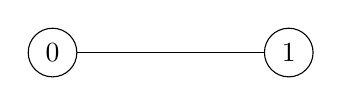
\begin{tikzpicture}[every node/.style={circle, draw, minimum size=0.5cm}]
            \node (A) at (0,0) {0};
            \node (B) at (3,0) {1};
        
            \draw (A) -- (B);
        \end{tikzpicture}
    }
    \item {
        $H_2$ \par
        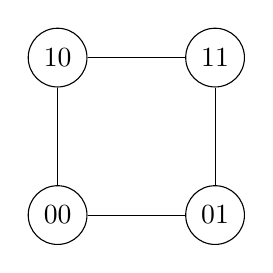
\begin{tikzpicture}[every node/.style={circle, draw, minimum size=0.5cm}]
            \node (A) at (0, 0) {00};
            \node (B) at (2, 0) {01};
            \node (C) at (2, 2) {11};
            \node (D) at (0, 2) {10};
        
            \draw (A) -- (B);
            \draw (B) -- (C);
            \draw (C) -- (D);
            \draw (D) -- (A);
        \end{tikzpicture}
    }
    \item {
        $H_3$ \par
        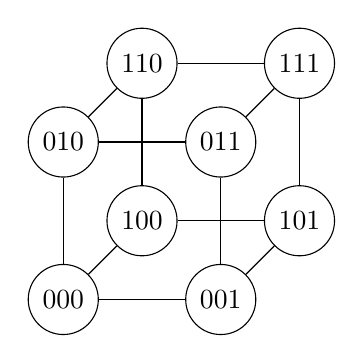
\begin{tikzpicture}[every node/.style={circle, draw, minimum size=0.5cm}]
            % Back face
            \node (000) at (0, 0) {000};
            \node (001) at (2, 0) {001};
            \node (011) at (2, 2) {011};
            \node (010) at (0, 2) {010};
            \node (100) at (1, 1) {100};
            \node (101) at (3, 1) {101};
            \node (111) at (3, 3) {111};
            \node (110) at (1, 3) {110};
        
            \draw (000) -- (001);
            \draw (001) -- (011);
            \draw (011) -- (010);
            \draw (010) -- (000);
            \draw (100) -- (101);
            \draw (101) -- (111);
            \draw (111) -- (110);
            \draw (110) -- (100);
            \draw (000) -- (100);
            \draw (001) -- (101);
            \draw (011) -- (111);
            \draw (010) -- (110);
        \end{tikzpicture}
    }
\end{itemize}
\end{multicols}

\subsection{Clique, independence and domination numbers}

\begin{dd}
    A clique is a subgraph of $G$ isomorphic to a complete graph. The \textbf{clique number $\omega(G)$} of $G$ is the size of the largest clique in $G$. 
    \begin{itemize}
        \item $\omega(H_n) = 2$
        \item $\omega(K_n) = n$
        \item $\omega(P_n) = 2$
    \end{itemize}
\end{dd}

\begin{dd}
    Independent set of a graph $G$ is a subset of its verices such that no two vertices in the subset are connected by an edge. The number of vertices in the maximum independent set is called the \textbf{independence number $\alpha(G)$}.
    \begin{itemize}
        \item $\alpha(C_n) = \left\lfloor \frac{n}{2} \right\rfloor$
        \item $\alpha(K_n) = 1$
        \item $\alpha(P_n) = \left\lfloor \frac{n + 1}{2} \right\rfloor$
    \end{itemize}
\end{dd}

\begin{dd}
    A domination set of a graph $G$ is a subset $S$ of vertices such that any vertex $v \in V(G)$ either belongs to $S$ or is adjacent to one of its vertices. Number of vertices in a minimum domination set is called the \textbf{domination number $\gamma(G)$} of $G$.
    \begin{itemize}
        \item $\gamma(C_n) = \left\lceil \frac{n}{3} \right\rceil$
        \item $\gamma(K_n) = 1$
        \item $\gamma(P_n) = \left\lceil \frac{n}{3} \right\rceil$
    \end{itemize}
\end{dd}

\subsection{Graph products}

\begin{dd}
    \textbf{The carthesian product} of $G$ and $H$ is the graph $G\ \square\ H$ with vertex set $V(G\ \square\ H) = V(G) \times V(H)$. Two vertices $(g_1, h_1)$ and $(g_2, h_2)$ are adjacent precisely if either $g_1 = g_2$ and $h_1h_2 \in E(H)$, or $g_1g_2 \in E(G)$ and $h_1 = h_2$.
    \begin{enumerate}
        \item $|V(G\ \square\ H)| = |V(G)| \cdot |V(H)|$
        \item $|E(G\ \square\ H)| = |V(G)| \cdot |E(H)| + |V(H)| \cdot |E(G)|$
        \item $\diam(G \ \square\ H) = \diam(G) + \diam(H)$
    \end{enumerate}
    \begin{multicols}{2}
    \begin{itemize}
        \item {
            $P_2\ \square\ P_2$ \par
            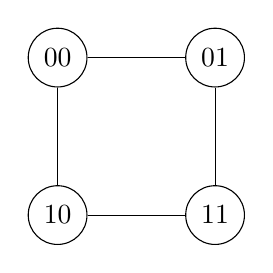
\begin{tikzpicture}[every node/.style={circle, draw, minimum size=0.5cm}]
                \node (A) at (0,0) {10};
                \node (B) at (2,0) {11};
                \node (C) at (0,2) {00};
                \node (D) at (2,2) {01};
            
                \draw (A) -- (B);
                \draw (A) -- (C);
                \draw (B) -- (D);
                \draw (C) -- (D);
            \end{tikzpicture}
        }
        \item {
            $P_2\ \square\ P_3$ \par
            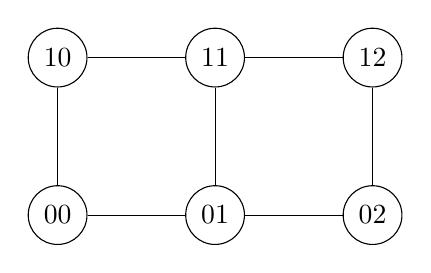
\begin{tikzpicture}[every node/.style={circle, draw, minimum size=0.5cm}]
                \node (A) at (0,0) {00};
                \node (B) at (2,0) {01};
                \node (C) at (4,0) {02};
                \node (D) at (0,2) {10};
                \node (E) at (2,2) {11};
                \node (F) at (4,2) {12};
            
                \draw (A) -- (B);
                \draw (B) -- (C);
                \draw (D) -- (E);
                \draw (E) -- (F);
                \draw (A) -- (D);
                \draw (B) -- (E);
                \draw (C) -- (F);
            \end{tikzpicture}
        }
    \end{itemize}
    \end{multicols}
\end{dd}

\begin{dd}
    \textbf{The direct product} of $G$ and $H$ is the graph $G \times H$ with vertex set $V(G \times H) = V(G) \times V(H)$. Two vertices $(g_1, h_1)$ and $(g_2, h_2)$ are adjacent precisely if $g_1g_2 \in E(G)$ and $h_1h_2 \in E(H)$.
    \begin{enumerate}
        \item $|V(G \times H)| = |V(G)| \cdot |V(H)|$
        \item $|E(G \times H)| = 2 \cdot |E(G)| \cdot |E(H)|$
        \item $G_1 \times (G_2 + G_3) = G_1 \times G_2 + G_1 \times G_3$
    \end{enumerate}
    \begin{multicols}{2}
    \begin{itemize}
        \item {
            $P_2 \times P_2$ \par
            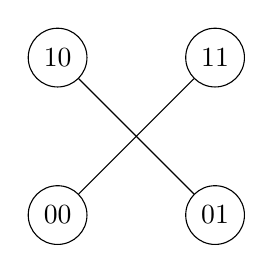
\begin{tikzpicture}[every node/.style={circle, draw, minimum size=0.5cm}]
                \node (A) at (0,0) {00};
                \node (B) at (2,0) {01};
                \node (C) at (0,2) {10};
                \node (D) at (2,2) {11};
            
                \draw (A) -- (D);
                \draw (B) -- (C);
            \end{tikzpicture}
        }
        \item {
            $P_2 \times P_3$ \par
            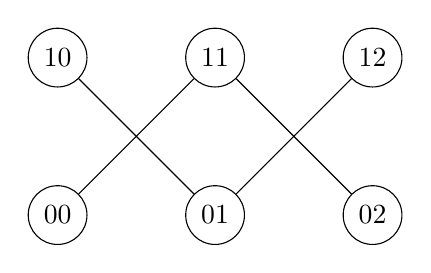
\begin{tikzpicture}[every node/.style={circle, draw, minimum size=0.5cm}]
                \node (A) at (0,0) {00};
                \node (B) at (2,0) {01};
                \node (C) at (4,0) {02};
                \node (D) at (0,2) {10};
                \node (E) at (2,2) {11};
                \node (F) at (4,2) {12};
            
                \draw (A) -- (E);
                \draw (B) -- (D);
                \draw (B) -- (F);
                \draw (C) -- (E);
            \end{tikzpicture}
        }
    \end{itemize}
    \end{multicols}
\end{dd}

If $G_1, \dots, G_k$ are finite non empty graphs, then their direct product is the graph $G_1 \times \dots \times G_k = \times_{i = 1}^k G_i$ with vertex set $V(\times_{i = 1}^k G_i) = \{(x_1, \dots, x_k): x_i \in V(G_i)\}$ and for which vertices $(x_1, \dots, x_k)$ and $(y_1, \dots, y_k)$ are adjacent precisely if $\forall i \in \{1, \dots, k\}\ x_iy_i \in E(G_i)$.

\begin{dd}
    \textbf{The strong product} of $G$ and $H$ is the graph $G \boxtimes H$ with vertex set $V(G \boxtimes H) = V(G) \times V(H)$ and the edges set $E(G \boxtimes H) = E(G\ \square\ H) \cup E(G \times H)$.
    \begin{enumerate}
        \item $|V(G \boxtimes H)| = |V(G)| \cdot |V(H)|$
        \item $|E(G \boxtimes H)| = |V(G)| \cdot |E(H)| + |V(H)| \cdot |E(G)| + 2 \cdot |E(G)| \cdot |E(H)|$
        \item $K_n \boxtimes K_m \cong K_{nm}$
        \item $K_1 \boxtimes G \cong G$
    \end{enumerate}
    \begin{multicols}{2}
    \begin{itemize}
        \item {
            $P_2 \boxtimes P_2$ \par
            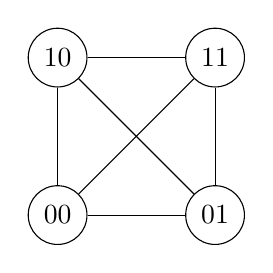
\begin{tikzpicture}[every node/.style={circle, draw, minimum size=0.5cm}]
                \node (A) at (0,0) {00};
                \node (B) at (2,0) {01};
                \node (C) at (0,2) {10};
                \node (D) at (2,2) {11};
            
                \draw (A) -- (D);
                \draw (B) -- (C);
                \draw (A) -- (B);
                \draw (A) -- (C);
                \draw (B) -- (D);
                \draw (C) -- (D);
            \end{tikzpicture}
        }
        \item {
            $P_2 \boxtimes P_3$ \par
            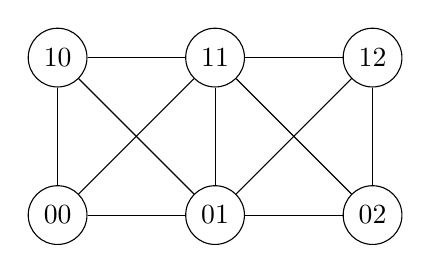
\begin{tikzpicture}[every node/.style={circle, draw, minimum size=0.5cm}]
                \node (A) at (0,0) {00};
                \node (B) at (2,0) {01};
                \node (C) at (4,0) {02};
                \node (D) at (0,2) {10};
                \node (E) at (2,2) {11};
                \node (F) at (4,2) {12};
            
                \draw (A) -- (E);
                \draw (B) -- (D);
                \draw (B) -- (F);
                \draw (C) -- (E);
                \draw (A) -- (B);
                \draw (B) -- (C);
                \draw (D) -- (E);
                \draw (E) -- (F);
                \draw (A) -- (D);
                \draw (B) -- (E);
                \draw (C) -- (F);
            \end{tikzpicture}
        }
    \end{itemize}
    \end{multicols}
\end{dd}

\noindent All products above are \textbf{commutative} and \textbf{associative}, meaning the following relations hold:
\begin{enumerate}
    \item $G_1 \star G_2 \cong G_2 \star G_1$
    \item $(G_1 \star G_2) \star G_3 \cong G_1 \star (G_2 \star G_3)$
\end{enumerate}

\subsection{Graph colouring}

\begin{dd}
    The minimum value $k$ such that $V(G)$ can be positioned into $k$ classes $V_1, V_2, \dots, V_k$ for which $\forall u, v \in V_i(G) \iff uv \notin E(G)$ is called the (vertex) \textbf{chromatic number} of $G$ and denoted $\chi(G)$. \\
    It's the minimum number of colours in a vertex colouring of $G$ - we colour each graph in such way that adjacent vertices have different colours.
    \begin{itemize}
        \item $\chi(G) \geq 2 \iff E(G) \neq \emptyset$
        \item $\chi(G) \geq 3 \iff G$ contains an odd cycle
        \item $\chi(G) = n \iff G \cong K_n$
        \item $\chi(G) = 2 \iff G$ is a bipartite graph
    \end{itemize}
\end{dd}

\subsubsection{Greedy algorithm}
\begin{enumerate}
    \item Order vertices of a graph: $x_1, \dots, x_n$
    \item {
        Colour them one by one:
        $x_1 \mapsto 1$, $x_2 \mapsto \begin{cases}
            1 & \text{if } x_1x_2 \notin E(G) \\
            2 & \text{otherwise}
        \end{cases}$, and so on...
    }
\end{enumerate}

\begin{theorem}
    Let $G$ be a graph and $\Delta(G) = \max\limits_{v \in V(G)}\deg v$, then: $\omega(G) \leq \chi(G) \leq \Delta(G) + 1$
\end{theorem}

\begin{prop}
    If $G$ is a connected, non-regular graph then $\chi(G) \leq \Delta(G)$.
\end{prop}

\begin{prop}
    Let $G$ be a connected planar graph. Then $\exists v \in V(G):\ \deg v \leq 5$.
\end{prop}

\begin{prop}
    Every planar graph is 4-colourable.
\end{prop}

\subsubsection{Examples}
\begin{multicols}{2}
\begin{itemize}
    \item {
        $K_6$ with chromatic number $\chi(K_6) = 6$ \par
        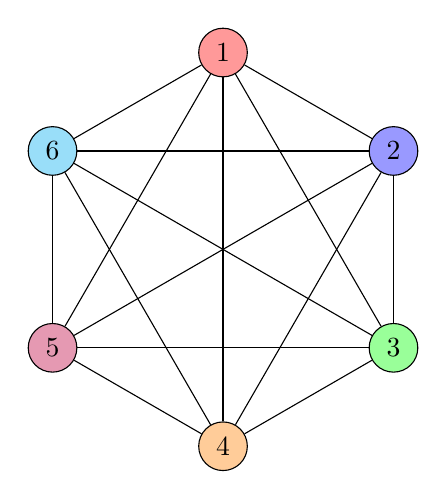
\begin{tikzpicture}[every node/.style={circle, draw, minimum size=0.5cm}]
            \node[fill=red!40]    (A) at (90:2.5cm) {1};
            \node[fill=blue!40]   (B) at (30:2.5cm) {2};
            \node[fill=green!40]  (C) at (-30:2.5cm) {3};
            \node[fill=orange!40] (D) at (-90:2.5cm) {4};
            \node[fill=purple!40] (E) at (-150:2.5cm) {5};
            \node[fill=cyan!40]   (F) at (150:2.5cm) {6};
        
            \draw (A) -- (B);
            \draw (A) -- (C);
            \draw (A) -- (D);
            \draw (A) -- (E);
            \draw (A) -- (F);
            \draw (B) -- (C);
            \draw (B) -- (D);
            \draw (B) -- (E);
            \draw (B) -- (F);
            \draw (C) -- (D);
            \draw (C) -- (E);
            \draw (C) -- (F);
            \draw (D) -- (E);
            \draw (D) -- (F);
            \draw (E) -- (F);
        \end{tikzpicture}
    }
    \item {
        $K_{4,4}$ with chromatic number $\chi(K_{4,4}) = 2$ \par
        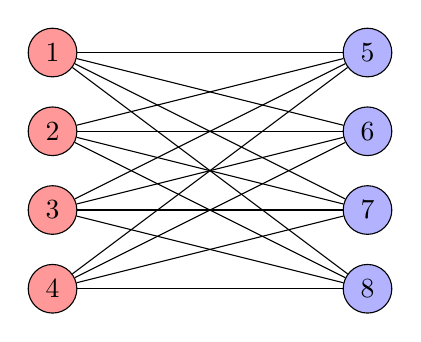
\begin{tikzpicture}[every node/.style={circle, draw, minimum size=0.5cm}]
            \node[fill=red!40]   (A1) at (0,3) {1};
            \node[fill=red!40]   (A2) at (0,2) {2};
            \node[fill=red!40]   (A3) at (0,1) {3};
            \node[fill=red!40]   (A4) at (0,0) {4};
        
            \node[fill=blue!30]  (B1) at (4,3) {5};
            \node[fill=blue!30]  (B2) at (4,2) {6};
            \node[fill=blue!30]  (B3) at (4,1) {7};
            \node[fill=blue!30]  (B4) at (4,0) {8};
        
            \draw (A1) -- (B1);
            \draw (A1) -- (B2);
            \draw (A1) -- (B3);
            \draw (A1) -- (B4);
        
            \draw (A2) -- (B1);
            \draw (A2) -- (B2);
            \draw (A2) -- (B3);
            \draw (A2) -- (B4);
        
            \draw (A3) -- (B1);
            \draw (A3) -- (B2);
            \draw (A3) -- (B3);
            \draw (A3) -- (B4);
        
            \draw (A4) -- (B1);
            \draw (A4) -- (B2);
            \draw (A4) -- (B3);
            \draw (A4) -- (B4);
        \end{tikzpicture}
    }
\end{itemize}
\end{multicols}

\newpage
\section{Lexicographic product, prime graphs and distances}

\subsection{Lexicographic (wreath) product}

\begin{dd}
    \textbf{The lexicographic (or wreath) product} of $G$ and $H$ is the graph $G\ \circ\ H$ with vertex set $V(G\ \circ\ H) = V(G) \times V(H)$. Two vertices $(g_1, h_1)$ and $(g_2, h_2)$ are adjacent precisely if either $g_1g_2 \in E(G)$, or $h_1h_2 \in E(H)$ and $g_1 = g_2$.
    \begin{enumerate}
        \item $|V(G\ \circ\ H)| = |V(G)| \cdot |V(H)|$
        \item $|E(G\ \circ\ H)| = |E(G)| \cdot |V(H)|^2 + |V(G)| \cdot |E(H)|$
        \item $K_n \circ K_m \cong K_{nm}$
        \item $K_1 \circ G \cong G$
        \item $G \circ K_1 \cong G$
        \item $(G \cup H) \circ K \cong G \circ K \cup H \circ K$
        \item $\overline{G} \circ \overline{H} \cong \overline{G \circ H}$
        \item $\diam(G \circ H) = \max\bigl\{\diam(G), min\{\diam(H), 2\}\bigr\}$
    \end{enumerate}
    \begin{multicols}{2}
    \begin{itemize}
        \item {
            $P_2\ \circ\ C_3$ \par
            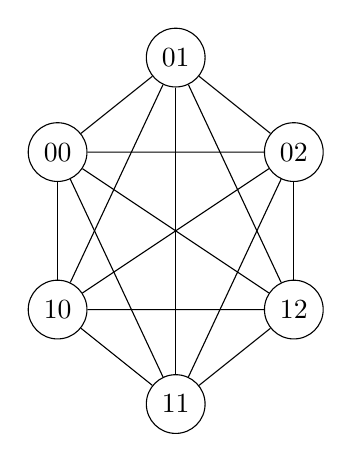
\begin{tikzpicture}[every node/.style={circle, draw, minimum size=0.5cm}]
                \node (A0) at (0,2) {00};
                \node (A1) at (1.5,3.2) {01};
                \node (A2) at (3,2) {02};

                \node (B0) at (0,0) {10};
                \node (B1) at (1.5,-1.2) {11};
                \node (B2) at (3,0) {12};

                \draw (A0) -- (A1) -- (A2) -- (A0);
                \draw (B0) -- (B1) -- (B2) -- (B0);

                \foreach \a in {A0, A1, A2}
                    \foreach \b in {B0, B1, B2}
                        \draw (\a) -- (\b);
            \end{tikzpicture}
        }
        \item {
            $P_2\ \circ\ P_3$ \par
            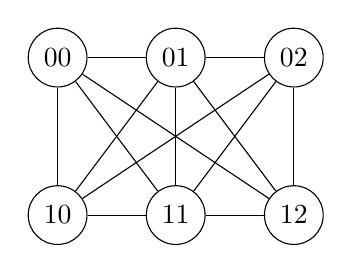
\begin{tikzpicture}[every node/.style={circle, draw, minimum size=0.5cm}]
                \node (A0) at (0,2) {00};
                \node (A1) at (1.5,2) {01};
                \node (A2) at (3,2) {02};
                \node (B0) at (0,0) {10};
                \node (B1) at (1.5,0) {11};
                \node (B2) at (3,0) {12};

                \draw (A0) -- (A1) -- (A2);
                \draw (B0) -- (B1) -- (B2);

                \foreach \a in {A0, A1, A2}
                    \foreach \b in {B0, B1, B2}
                        \draw (\a) -- (\b);
            \end{tikzpicture}
        }
    \end{itemize}
    \end{multicols}
\end{dd}

\subsubsection{Distances in the lexicographic product}
Suppose that $(g_1, h_1), (g_2, h_2) \in V(G \circ H)$. Then: \\
$d_{G \circ H}\bigl((g_1, h_1), (g_2, h_2)\bigr) = \begin{cases}
    d_G(g_1, g_2) & \text{if } g_1 \neq g_2 \\
    d_H(h_1, h_2) & \text{if } g_1 = g_2 \text{ and } \deg_G(g_1) = 0 \\
    \min\{d_H(h_1, h_2), 2\} & \text{if } g_1 = g_2 \text{ and } \deg_G(g_1) \neq 0 \\
\end{cases}$

\begin{corollary}
    Suppose that $\mathbbm{x} = (x_1, \dots, x_k)$ and $\mathbbm{y} = (y_1, \dots, y_k)$ are vertices of graph $G = G_1 \circ \dots \circ G_k$. Let $i$ be the smallest index for which $x_i \neq y_i$. Then: \\
    $d_G(\mathbbm{x}, \mathbbm{y}) = \begin{cases}
        d_{G_i}(x_i, y_i) & \text{if } \forall l = 1, \dots, i \quad \deg_{G_l}(x_l) = 0 \text{ and } x_1 = y_1, \dots, x_{i - 1} = y_{i - 1} \\
        \min\{d_{G_i}(x_i, y_i), 2\} & \text{if } \exists l = 1, \dots, i \quad \deg_{G_l}(x_l) \neq 0 \text{ and } x_1 = y_1, \dots, x_{i - 1} = y_{i - 1} \\
    \end{cases}$
\end{corollary}

\begin{corollary}
    The product $G = G_1 \circ \dots \circ G_k$ of nontrivial graphs is connected $\iff G_1$ is connected.
\end{corollary}

\subsection{Prime factor decompositions}

\begin{dd}
    A graph is \textbf{prime} with respect to a given product if it's nontrivial and can't be represented as a product of two nontrivial graphs: \\
    $G$ is prime if $G = G_1\ \square\ G_2 \implies G_1 \cong K_1 \lor G_2 \cong K_1$
\end{dd}

\begin{prop}
    Every nontrivial graph $G$ has a prime factor decomposition with respect to the carthesian product. The number of prime factors is at most $\log_2|V(G)|$
\end{prop}

\begin{theorem}
    The prime factorization is not unique for the carthesian product in the class of possibly disconnected simple graphs.
\end{theorem}

\begin{theorem}[Sabidussi-Vizing]
    Every connected graph has a unique reprezentation as a product of prime graphs, up to isomorphism and the order of the factors.
\end{theorem}

\begin{corollary}
    Suppose there is an isomorphism $\phi:\ G_1\ \square\ \dots\ \square\ G_k\ \to\ H_1\ \square\ \dots\ \square\ H_k$ where each $G_i$ and $H_i$ are prime. Then the vertices of the graph $H_i$ can be relabeled such that $\phi(x_1, \dots, x_k) = (x_{\sigma(1)}, \dots, x_{\sigma(k)})$ for permutation $\sigma$ of $\{1, \dots, k\}$.
\end{corollary}

\begin{theorem}
    Let $G, H, K$ be finite simple graphs. Suppose that $K$ is not empty. Then $G\ \square\ K \cong H\ \square\ K \implies G \cong H$.
\end{theorem}

\begin{prop}
    Suppose that $(g_1, h_1), (g_2, h_2) \in V(G\ \square\ H)$. Then: \\
    $d_{G \square H}\bigl((g_1, h_1), (g_2, h_2)\bigr) = d_G(g_1, g_2) + d_H(h_1, h_2)$.
\end{prop}

\begin{corollary}
    Suppose that $\mathbbm{x} = (x_1, \dots, x_k)$ and $\mathbbm{y} = (y_1, \dots, y_k)$ are distinct vertices of graph $G = G_1\ \square\ \dots\ \square\ G_k$. Then: \\
    $d_G(\mathbbm{x}, \mathbbm{y}) = \sum\limits_{i = 1}^k d_{G_i}(x_i, y_i)$
\end{corollary}

\begin{corollary}
    The carthesian product of graphs is connected $\iff$ every factor of the graph is connected.
\end{corollary}

\subsection{Distances in the direct product}

\begin{prop}
    Suppose $(g_1, h_1)$ and $(g_2, h_2)$ are vertices of a direct product $G \times H$ and $n$ is an integer for which $G$ has a $g_1,g_2$-walk of length $n$ and $H$ has an $h_1,h_2$-walk of length $n$. Then $G \times H$ has a walk of length $n$ from $(g_1, h_1)$ to $(g_2, h_2)$. The smallest such $n$ (if it exists) equals $d_{G \times H}\bigl((g_1, h_1), (g_2, h_2)\bigr)$. If no such $n$ exists, then $d_{G \times H}\bigl((g_1, h_1), (g_2, h_2)\bigr) = \infty$.
\end{prop}

\begin{prop}
    Suppose $\mathbbm{x}$ and $\mathbbm{y}$ are vertices of $G = \times_{i = 1}^k G_i$. Then: \\
    $d_G(\mathbbm{x}, \mathbbm{y}) = \min\{n \in \mathbb{N}:\ \text{each factor } G_i \text{ has a walk of length } n \text{ from } p_i(\mathbbm{x}) \text{ to } p_i(\mathbbm{y})\}$ \\
    Where it is understood that $d_G(\mathbbm{x}, \mathbbm{y}) = \infty$ if no such $n$ exists.
\end{prop}

\begin{theorem}[Weichsel's theorem]
    Suppose $G$ and $H$ are connected finite nontrivial graphs. If at least one of $G$ or $H$ has an odd cycle, then $G \times H$ is connected. If both $G$ and $H$ are bipartite, then $G \times H$ has exactly two components.
\end{theorem}

\begin{corollary}
    A direct product of connected nontrivial finite graphs is connected $\iff$ at most one of the factors is bipartite. \\
    The product has $2k - 1$ components, where $k$ is the number of bipartite factors.
\end{corollary}

\end{document}